\documentclass{article}
\usepackage{amsmath}
\usepackage{amssymb}
\usepackage[margin=1.2in]{geometry}
\usepackage{graphicx}

\begin{document}

\title{Numerical Analysis HW \#5}
\author{Ozaner Hansha}
\date{May 2, 2019}
\maketitle

\section*{Problem 1}
\subsection*{Part a}
\textbf{Problem:} Use Euler's method with step size $h=\frac{1}{2}$ to approximate $y\left(\frac{1}{2}\right)$ and $y(1)$ where $y(x)$ is the solution to the following IVP:

$$y'=1-8xy\ \ \ \ \ \ \ \ \ \  y(0)=0$$
\\
\textbf{Solution:} Recall that Euler's method is given by the following iteration for each equally spaced node $x_i$:

$$y_{i+1}=y_i+hf(x_i,y_i)$$

For $y\left(\frac{1}{2}\right)$ our interval is $[0,\frac{1}{2}]$. This gives us only one iteration step at $x_1=\frac{1}{2}$:

$$y_1=y_0+hf(x_0,y_0)=0+\frac{1}{2}(1-8(0)(0))=\boxed{\frac{1}{2}\approx y\left(\frac{1}{2}\right)}$$

For $y(1)$ our interval is $[0,1]$. gives us one more iteration step for $x_2=1$:

$$y_2=y_1+hf(x_1,y_1)=\frac{1}{2}+\frac{1}{2}\left(1-8\left(\frac{1}{2}\right)\left(\frac{1}{2}\right)\right)=\boxed{0\approx y(1)}$$

\subsection*{Part b}
\textbf{Problem:} Repeat part a, but with a Taylor series method of order two.
\\\\
\textbf{Solution:} Recall that the Taylor Series method of degree two is given by the following iteration for each equally spaced node $x_i$:

$$y_{i+1}=y_i+hf(x_i,y_i)+\frac{h^2}{2}\left[\frac{\partial f}{\partial x}+\frac{\partial f}{\partial y}f\right](x_i,y_i)$$

To solve this method explicitly, we must first compute the summands of $\frac{\partial f}{\partial x}+\frac{\partial f}{\partial y}f$:

\begin{align*}
  \frac{\partial f}{\partial x}&=\frac{\partial}{\partial x}1-8xy=-8y\\
  \frac{\partial f}{\partial y}f&=\left(\frac{\partial}{\partial y}1-8xy\right)(1-8xy)\\
  &=-8x(1-8xy)\\
  &=64x^2y-8x
\end{align*}

The sum of these terms is then:

$$\frac{\partial f}{\partial x}+\frac{\partial f}{\partial y}f=(-8y)+(64x^2y-8x)=64x^2y-8x-8y$$

Giving us a final iteration method of:

$$y_{i+1}=y_i+h(1-8x_iy_i)+\frac{h^2}{2}(64x_i^2y_i-8x_i-8y_i)$$


For $y\left(\frac{1}{2}\right)$ our interval is $[0,\frac{1}{2}]$. This gives us only one iteration step at $x_1=\frac{1}{2}$:

\begin{align*}
y_1&=y_0+h(1-8x_0y_0)+4h^2(8x_0^2y_0-x_0-y_0)\\
&=0+\left(\frac{1}{2}\right)(1-8(0)(0))+4\left(\frac{1}{2}\right)^2(8(0)^2(0)-(0)-(0))\\
&=\boxed{\frac{3}{2}\approx y\left(\frac{1}{2}\right)}
\end{align*}

For $y(1)$ our interval is $[0,1]$. This gives us one more iteration step for $x_2=1$:

\begin{align*}
  y_2&=y_1+h(1-8x_1y_1)+4h^2(8x_1^2y_1-x_1-y_1)\\
  &=\frac{3}{2}+\left(\frac{1}{2}\right)\left(1-8\left(\frac{1}{2}\right)\left(\frac{3}{2}\right)\right)+4\left(\frac{1}{2}\right)^2\left(8\left(\frac{1}{2}\right)^2\left(\frac{3}{2}\right)-\left(\frac{1}{2}\right)-\left(\frac{3}{2}\right)\right)\\
  &=\boxed{0\approx y(1)}
\end{align*}

\subsection*{Part c}
\textbf{Problem:} Repeat part a, but with Heun's method.
\\\\
\textbf{Solution:} Recall that Heun's method is given by:

$$y_{i+1}=y_i+\frac{h}{2}[f(x_i,y_i)+f(x_{i+1},\tilde y_{i+1})]$$

Where $\tilde y_{i+1}$ is an approximation of $y_{i+1}$:

$$\tilde y_{i+1}=y_i+hf(x_i,y_i)$$

For $y\left(\frac{1}{2}\right)$ we have one iteration at $x_1=\frac{1}{2}$. First we calculate $\tilde y_1$:

\begin{align*}
  \tilde y_1&=y_0+hf(x_0,y_0)\\
  &=0+\frac{1}{2}(1-8(0)(0))=\frac{1}{2}
\end{align*}

Now we can calculate our approximation $y_1$:

\begin{align*}
  y_1&=y_0+\frac{h}{2}[f(x_0,y_0)+f(x_1,\tilde y_1)]\\
  &=0+\frac{1}{2}\left(\frac{1}{2}\right)\left[(1-8(0)(0))+\left(1-8\left(\frac{1}{2}\right)\left(\frac{1}{2}\right)\right)\right]\\
  &=\boxed{0\approx y\left(\frac{1}{2}\right)}
\end{align*}

And for $y(1)$ we have one more iteration at $x_2=1$. First we calculate $\tilde y_2$:

\begin{align*}
  \tilde y_2&=y_1+hf(x_1,y_1)\\
  &=0+\frac{1}{2}\left(1-8\left(\frac{1}{2}\right)(0)\right)=\frac{1}{2}
\end{align*}

Now we can calculate our approximation $y_2$:

\begin{align*}
  y_2&=y_1+\frac{h}{2}[f(x_1,y_1)+f(x_2,\tilde y_2)]\\
  &=0+\frac{1}{2}\left(\frac{1}{2}\right)\left[\left(1-8\left(\frac{1}{2}\right)(0)\right)+\left(1-8(1)\left(\frac{1}{2}\right)\right)\right]\\
  &=\frac{1}{4}(1-3)=\boxed{-\frac{1}{2}\approx y(1)}
\end{align*}

\section*{Problem 2}
\subsection*{Part a}
\textbf{Problem:} Using the same IVP as Problem 1, approximate $y(5)$ over the interval $[0,5]$ with a step size of $h=0.1$ using Euler's method in MATLAB. Then plot $y$ over the interval.
\\\\
\textbf{Solution:} The approximation is $y(5)\approx 0.025118547520984$ and the plot is given below:

\begin{center}
  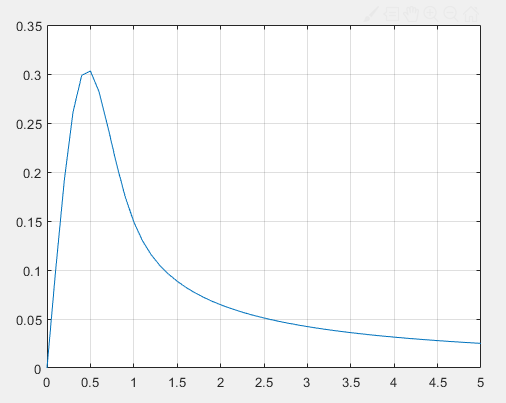
\includegraphics[scale=0.7]{plot1.png}
\end{center}


\subsection*{Part b}
\textbf{Problem:} Do the same as part a, but approximate $y(5.9)$ on the interval $[0,5.9]$. Is the numerical solution accurate?
\\\\
\textbf{Solution:} The approximation is $y(5.9)\approx 0.300553327482678$ and the plot is given below:

\begin{center}
  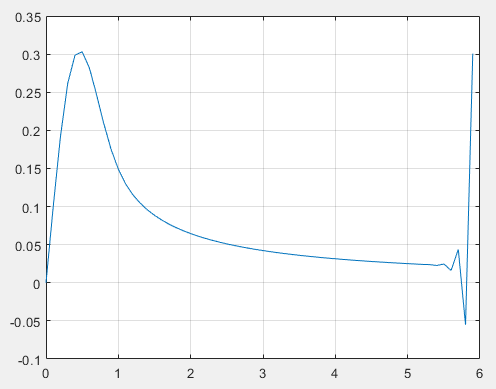
\includegraphics[scale=0.7]{plot2.png}
\end{center}

The numerical solution is indeed \emph{not} accurate. The true solution, while not elementary, is smooth and is decreasing as $x\to\infty$. This is not reflected on our numerical plot. In particular the huge spike at the end means our approximation of $0.3005$ is wildly off. The true solution is approximately $0.0212634$.

\end{document}
